Optimal control -which is playing an increasingly important role in
the design of modern systems- has as its aim the optimization,
in some defined sense, of physical processes. 
More specifically, the
objective of optimal control is to determine the control signals
that will cause a process to satisfy the physical constraints and at
the same time minimize or maximize some performance criterion
\cite{Kirk1970}.

The formulation of an optimal control problem requires:

\begin{itemize}
\item[-] A mathematical model.
\item[-] A neural network.
\item[-] A performance functional.
\item[-] A training strategys.
\end{itemize}

\subsection*{Mathematical model}\index{mathematical model}
\index{state variable}
\index{control variable}
\index{state equation}
\index{algebraic operator}
\index{differential operator}
\index{forcing term}

The model of a process is a mathematical description that
adequately predicts the response of the physical system to all
anticipated inputs.

A mathematical model (or state equation) contains state variables and control variables. 
Mathematical models can be expressed as all algebraic, ordinary differential and partial differential equations. 
However, many optimal control problems in the literature are based on mathematical models described by a system of ordinary differential equations together with their respective initial conditions, representing a dynamical model of the system. 
Integration here is usually performed with the Runge-Kutta-Fehlberg method.

\subsection*{Neural network}
\index{input constraint}
\index{control constraint}
\index{state constraint}
\index{boundary condition}
\index{lower and upper bounds}
\index{admissible control}

A neural network is used to represent the control variables. 
The number of inputs is usually one, which represents the time, and the number of outputs is normally small, representing the control variables. 
Although the number of hidden layers and the sizes of each are design variables, that is not a critical issue in optimal control. 
Indeed, this class of problems are regarded as being well-possed, 
and a sufficient complexity for the function space selected is generally enough. 

Figure \ref{NeuralNetworkOptimalControlFigure} shows a neural network template for solving optimal control problems. 

\begin{figure}[h!]
\begin{center}
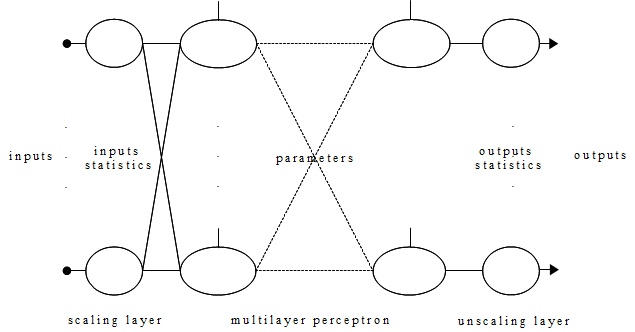
\includegraphics[width=1.2\textwidth]{optimal_control/neural_network_optimal_control.png}
\caption{Neural network for optimal control.}\label{NeuralNetworkOptimalControlFigure}
\end{center}
\end{figure}

An optimal control problem might be specified by a set of constraints on the control variables. 
Two important types of control constraints are boundary conditions and lower and upper bounds. 

If some outputs are specified for given
inputs, then the problem is said to include boundary
conditions. On the other hand, if some
control variables are restricted to fall in some interval, then the
problem is said to have lower and upper bounds.

Also, some optimal control problems need a neural network with associated independent parameters. 
The most common are those with free final time.

\subsection*{Performance functional}
\index{performance criterion, see objective functional}
\index{admissible state}

The performance functional of an optimal control problem always includes an objective term.
It might also include a regularization and a constraints terms,  

\begin{eqnarray}\nonumber
\text{Performance functional = objective term + regularization term + constraints term}. 
\end{eqnarray}

In certain cases the problem statement might clearly indicate which
objective criterion is to be selected, whereas in other cases that
selection is a subjective matter \cite{Kirk1970}.

The regularization term makes the control variables to have smoother shapes. 

State constraints are conditions that the physical system must
satisfy. This type of constraints vary according to the problem at
hand.

In this way, a control which satisfies all the control and state
constraints is called an admissible control \cite{Kirk1970}.

Similarly, a state which satisfies the state constraints is called
an admissible state \cite{Kirk1970}.

An optimal control is defined as one that minimizes or maximizes the
performance criterion, and the corresponding state is called an
optimal state. In this way, the problem of optimal control is formulated as a
variational problem \cite{Kirk1970}.

In general, the performance function, cannot be evaluated analytically. 
This makes that the gradient vector and the Hessian matrix can neither be computed analytically, and numerical differentiation must be used. 

\subsection*{Training strategy}

We have seen that the performance functional for optimal control problems might contain up to three terms: 
objective, regularization and constraints. On the other hand, in most of the cases, it cannot be computed analitycally. 
That makes that a single training algorithm might not fully converge if the solution is far away from the optimal one. 

Therefore, when solving optimal control problems, it is recommended to use an initialization training algorithm before the main training process. 
The form of the training strategy is therefore as follows:

\begin{eqnarray}\nonumber
\text{Training strategy: initialization training algorithm, main training algorithm}. 
\end{eqnarray}

The initialization training algorithm is usually a zero order algorithm, such as random search or the evolutionary algorithm;
the main training algorithm might be a first order algorithm, such as conjugate gradient or the quasi-Newton method. 
